\documentclass{article}
\pagestyle{empty}

\usepackage[normalem]{ulem}

% set up page size and margins
%\usepackage[letterpaper,landscape,centering,margin=0.5in]{geometry}
%\usepackage[screen,centering,margin=0.5in]{geometry}
\usepackage[paperwidth=240mm,paperheight=180mm,centering,margin=0.5in]{geometry}

% this was recommended by psnfss2e.pdf
%\usepackage{textcomp}
%\usepackage{txfonts}
%\renewcommand{\rmdefault}{cm}
%\usepackage{lmodern}
%\usepackage[Symbol]{upgreek}
%\newcommand{\alphaup}{\upalpha}
%%% Upright Greek letters
\usepackage{amsfonts}
\DeclareSymbolFont{UPM}{U}{eur}{m}{n}
\SetSymbolFont{UPM}{bold}{U}{eur}{b}{n}
\DeclareMathSymbol{\upalpha}{0}{UPM}{"0B}
\DeclareMathSymbol{\upbeta}{0}{UPM}{"0C}
%\usepackage[math]{kurier}
%\renewcommand{\rmdefault}{cm}
\usepackage[T1]{fontenc}
\usepackage{cmbright}
%\usepackage{ccfonts}

%\usepackage{psfonts}

%\usepackage{helvet}
%\usepackage{avant}

\usepackage{url}

%% % from http://www.superstrate.net/useful/useful.html
%% \DeclareFontFamily{U}{euc}{}% I chose euc because the chart is called Euler cursive
%% \DeclareFontShape{U}{euc}{m}{n}{<-6>eurm5<6-8>eurm7<8->eurm10}{}%
%% \DeclareSymbolFont{AMSc}{U}{euc}{m}{n} % I chose AMSc because AMSa and AMSb are defined in the amsfonts-package
%% \DeclareMathSymbol{\alphaup}{\mathord}{AMSc}{11}

% scale up the fonts and space things correctly


%\linespread{2}

%% stolen from file `a0poster.cls', modified by RHK shifted font sizes
%% down three lines (and added three smaller sizes)
\renewcommand{\tiny}        {\fontsize{6.95}{8.68}\selectfont}    
\renewcommand{\scriptsize}  {\fontsize{8.33}{10.42}\selectfont}    
\renewcommand{\footnotesize}{\fontsize{10}{12.5}\selectfont}    
\renewcommand{\small}       {\fontsize{12}{14}\selectfont}    
\renewcommand{\normalsize}  {\fontsize{14.4}{18}\selectfont}  
\renewcommand{\large}       {\fontsize{17.28}{22}\selectfont} 
\renewcommand{\Large}       {\fontsize{20.74}{25}\selectfont} 
\renewcommand{\LARGE}       {\fontsize{24.88}{30}\selectfont} 
\renewcommand{\huge}        {\fontsize{26.5}{32}\selectfont} 
\renewcommand{\Huge}        {\fontsize{35.83}{45}\selectfont} 
\newcommand{\veryHuge}      {\fontsize{43}{54}\selectfont}    
\newcommand{\VeryHuge}      {\fontsize{51.6}{64}\selectfont}  
\newcommand{\VERYHuge}      {\fontsize{61.92}{77}\selectfont} 
%			    {\fontsize{74.3}{93}\selectfont}  
%			    {\fontsize{89.16}{112}\selectfont}
%			    {\fontsize{107}{134}\selectfont}  

% These colours are tried and tested for titles and headers. Don't
% over use color!
\usepackage{color}
\definecolor{DarkBlue}{rgb}{0.1,0.1,0.5}
\definecolor{Red}{rgb}{0.8,0.0,0.0}
\definecolor{Purple}{rgb}{0.8,0.0,0.8}
\definecolor{LightRed}{rgb}{1.0,0.0,0.0}
\definecolor{Cyan}{rgb}{0.0,0.9,0.9}
\definecolor{Magenta}{rgb}{0.9,0.0,0.9}
\definecolor{Green}{rgb}{0.0,0.9,0.0}
\definecolor{PicBlue}{rgb}{0.098,0.082,0.227}

%% stolen from http://www.edwardtufte.com/tufte/
\definecolor{ETYellow}{rgb}{1,1,0.953}

%% I've made it darker to calm the effect when projected on a large
%% screen
\definecolor{BGYellow}{rgb}{0.95,0.95,0.85}
% \definecolor{BGYellow}{rgb}{0.9,0.9,0.7}
%\pagecolor{BGYellow}

% see documentation for a0poster class for the size options here
\def\Head#1{\noindent\begin{center}{\Large\color{DarkBlue}#1}\end{center}}
\def\Important#1{\noindent{\color{Red} #1}}
\def\ImportantB#1{\noindent{ #1}}
\def\LHead#1{\noindent{\Large #1}}
\def\Title#1{\noindent\begin{center}{\Huge\color{Red}#1}\end{center}}
\def\Subtitle#1{\noindent\begin{center}{\huge\color{DarkBlue}#1}\end{center}}

% select the right font
%\renewcommand{\familydefault}{\sfdefault}

% The textpos package is necessary to position textblocks at arbitary 
% places on the page.
\usepackage[absolute,overlay]{textpos}

\usepackage{amsmath}
\usepackage{amssymb}

% Graphics to include graphics. Times is nice on posters, but you
% might want to switch it off and go for CMR fonts.
%\usepackage{graphics,wrapfig,times}
\usepackage{graphicx,wrapfig}

\TPGrid[0.5in,0.5in]{10}{10} % 2 cols of width 4.5, plus 1 gap of width 1

\parindent=0pt
\parskip=0.5\baselineskip

%\newcommand\ion[2]{#1{\scshape{#2}}} 
\newcommand\ion[2]{#1{\MakeUppercase{#2}}} 
\newcommand{\nH}{\ensuremath{n_\mathrm{H}}}
\newcommand{\Hn}{\ensuremath{\mathrm{HI}}}
\newcommand{\Hp}{\ensuremath{\mathrm{HII}}}
\newcommand{\Hen}{\ensuremath{\mathrm{HeI}}}
\newcommand{\Hep}{\ensuremath{\mathrm{HeII}}}
\newcommand{\Hepp}{\ensuremath{\mathrm{HeIII}}}
\newcommand{\logNH}{\ensuremath{\log(N_\mathrm{H}/\mathrm{cm}^{-2})}}

\begin{document}
\large

\pagecolor{white}
\begin{textblock}{10}(0,1)
\Title{Uncertainty versus Decisions}
\Subtitle{Some (false) dichotomies between\\ Astrophysics and Machine Learning}
\end{textblock}

\begin{textblock}{10}(0,5)

\Head{\large Roban Hultman Kramer}

\centering Hightable\\
{\small http://hightable.com}\\\vspace{0.1in}
a part of Gerson Lehrman Group\\
{\small http://gersonlehrmangroup.com}
\end{textblock}

$\;$

\vfill
\begin{center}
\small
\texttt{roban@astro.columbia.edu}\\
\texttt{http://roban.github.com/\\
}
\end{center}

%%%%%%%%%%%%%%%%%%%%%%%%%%%%%%%%%%%%%%%%%%%%%%%%%%%%%%%%%%%%%%%%%%%%%%%%%%%%%%
\
\clearpage
%%%%%%%%%%%%%%%%%%%%%%%%%%%%%%%%%%%%%%%%%%%%%%%%%%%%%%%%%%%%%%%%%%%%%%%%%%%%%%

\pagecolor{white}
\begin{textblock}{5}(0,0)
\centering {\huge Astrophysics}
\end{textblock}

\begin{textblock}{5}(5,0)
\centering {\huge Machine Learning}
\end{textblock}

\begin{textblock}{5}(0,1)\Large
\centering \textcolor{Red}{\VERYHuge Uncertainty} \vspace{0.5in}

Constraining Parameters  \vspace{0.5in} \\
\end{textblock}

\begin{textblock}{1}(4.5,0.75)
\centering {\Huge vs.\vspace{1in}}
\end{textblock}

\begin{textblock}{5}(5,1)\Large
\centering \textcolor{DarkBlue}{\VERYHuge Decisions}  \vspace{0.5in}

Making Predictions  \vspace{0.5in} \\

\end{textblock}


%%%%%%%%%%%%%%%%%%%%%%%%%%%%%%%%%%%%%%%%%%%%%%%%%%%%%%%%%%%%%%%%%%%%%%%%%%%%%%
\
\clearpage
%%%%%%%%%%%%%%%%%%%%%%%%%%%%%%%%%%%%%%%%%%%%%%%%%%%%%%%%%%%%%%%%%%%%%%%%%%%%%


\pagecolor{white}
\begin{textblock}{5}(0,0)
\centering {\huge Astrophysics}
\end{textblock}

\begin{textblock}{5}(5,0)
\centering {\huge Machine Learning}
\end{textblock}

\begin{textblock}{5}(0,1)\Large
\centering \textcolor{Red}{\VERYHuge Uncertainty} \vspace{0.1in}

Constraining Parameters  \vspace{0.1in} \\
\textcolor{Red}{\huge Example: MCMC}  \vspace{0.1in} \\
exploring parameter space\\
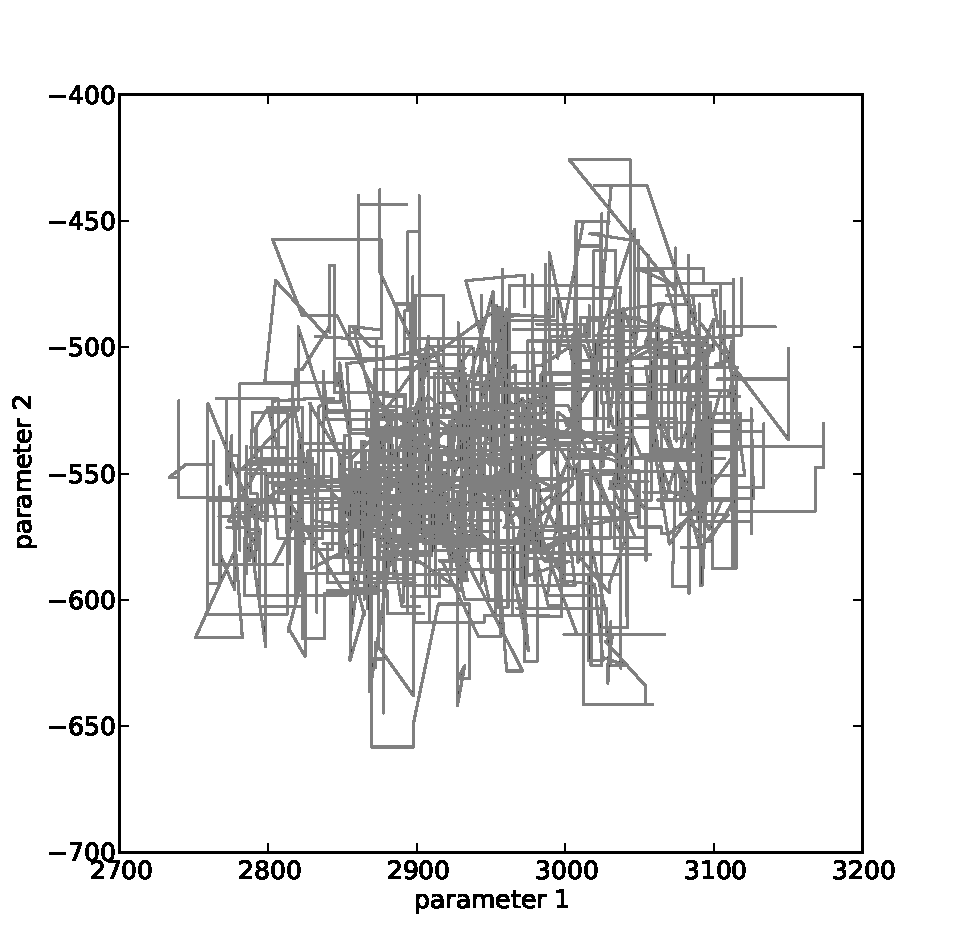
\includegraphics[width=4\TPHorizModule]{images/MCMC.pdf}
\end{textblock}

\begin{textblock}{1}(4.5,0.75)
\centering {\VERYHuge vs.\vspace{1in}}
\end{textblock}

\begin{textblock}{5}(5,1)\Large
\centering \textcolor{DarkBlue}{\VERYHuge Decisions}  \vspace{0.1in}

Making Predictions  \vspace{0.1in} \\
\textcolor{DarkBlue}{\huge Example: SVM}  \vspace{0.1in} \\
finding boundaries in feature space\\
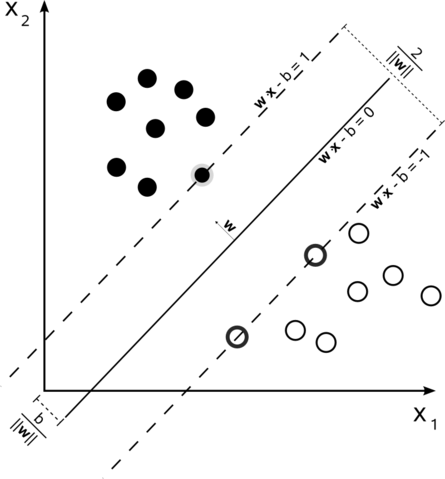
\includegraphics[width=4\TPHorizModule]{images/445px-Svm_max_sep_hyperplane_with_margin.png}
\\{\tiny Credit: Wikimedia Commons\\ \texttt{http://en.wikipedia.org/wiki/File:Svm\_max\_sep\_hyperplane\_with\_margin.png}}
\end{textblock}


%%%%%%%%%%%%%%%%%%%%%%%%%%%%%%%%%%%%%%%%%%%%%%%%%%%%%%%%%%%%%%%%%%%%%%%%%%%%%%
\
\clearpage
%%%%%%%%%%%%%%%%%%%%%%%%%%%%%%%%%%%%%%%%%%%%%%%%%%%%%%%%%%%%%%%%%%%%%%%%%%%%%


\pagecolor{white}
\begin{textblock}{5}(0,0)
\centering {\huge Astrophysics}
\end{textblock}

\begin{textblock}{5}(5,0)
\centering {\huge Machine Learning}
\end{textblock}

\begin{textblock}{5}(0,1)\Large
\centering \textcolor{Red}{\VERYHuge Uncertainty} \vspace{0.1in}

Constraining Parameters  \vspace{0.1in} \\
\textcolor{Red}{\huge Examples:}  \vspace{0.2in} \\
error bars\\
$p$-values\\
posterior distributions
\end{textblock}

\begin{textblock}{1}(4.5,0.75)
\centering {\VERYHuge vs.\vspace{1in}}
\end{textblock}

\begin{textblock}{5}(5,1)\Large
\centering \textcolor{DarkBlue}{\VERYHuge Decisions}  \vspace{0.1in}

Making Predictions  \vspace{0.1in} \\
\textcolor{DarkBlue}{\huge Examples:}  \vspace{0.2in} \\
$F_\beta$-scores\\
lift\\
ROC curves

\end{textblock}


%%%%%%%%%%%%%%%%%%%%%%%%%%%%%%%%%%%%%%%%%%%%%%%%%%%%%%%%%%%%%%%%%%%%%%%%%%%%%%
\
\clearpage
%%%%%%%%%%%%%%%%%%%%%%%%%%%%%%%%%%%%%%%%%%%%%%%%%%%%%%%%%%%%%%%%%%%%%%%%%%%%%


\pagecolor{white}
\begin{textblock}{5}(0,0)
\centering {\huge Astrophysics}
\end{textblock}

\begin{textblock}{5}(5,0)
\centering {\huge Machine Learning}
\end{textblock}

\begin{textblock}{5}(0,1)\Large
\centering \textcolor{Red}{\VERYHuge \sout{Uncertainty}}\\
\centering \textcolor{Red}{\VERYHuge Decisions} \vspace{0.1in}
\end{textblock}

\begin{textblock}{5}(5,1)\Large
\centering \textcolor{DarkBlue}{\VERYHuge Decisions}  \vspace{0.1in}
\end{textblock}


\begin{textblock}{1}(4.5,0.75)
\centering {\VERYHuge vs.\vspace{1in}}\vspace{0.1in}
\end{textblock}

\begin{textblock}{10}(0.0,2.5)
  \centering
{\Huge Counter Example}\vspace{0.1in}

\huge Planning observations and selecting targets
\end{textblock}


\begin{textblock}{5}(0,5)\Large\centering
\textbf{Examples:}\\
telescope time\\
budgets for instruments

(HST oversubscribed by $\approx 600\%$)

\end{textblock}

\begin{textblock}{5}(5,5)\Large\centering
\textbf{Examples:}\\
recommendation lists\\
marketing budgets\\
\end{textblock}

%%%%%%%%%%%%%%%%%%%%%%%%%%%%%%%%%%%%%%%%%%%%%%%%%%%%%%%%%%%%%%%%%%%%%%%%%%%%%%
\
\clearpage
%%%%%%%%%%%%%%%%%%%%%%%%%%%%%%%%%%%%%%%%%%%%%%%%%%%%%%%%%%%%%%%%%%%%%%%%%%%%%



\end{document}
